\documentclass[../main.tex]{subfiles}

\begin{document}

\begin{table}[!h]
    \begin{tabular}{rlllllll}
        \toprule
        participant &  \multicolumn{3}{l}{5} & \multicolumn{3}{l}{10} \\
              &                 model &     accuracy & balanced accuracy &                model &     accuracy & balanced accuracy \\
        \midrule
             niv &  logistic\_regression &  0.30 / 0.27 &       0.26 / 0.17 &             AdaBoost &  0.40 / 0.29 &       0.35 / 0.17 \\
          shiran &              bagging &  0.79 / 0.78 &       0.19 / 0.17 &           linear\_svm &  0.80 / 0.76 &       0.24 / 0.17 \\
             tal &        decision\_tree &  0.48 / 0.44 &       0.29 / 0.17 &              bagging &  0.50 / 0.39 &       0.39 / 0.17 \\
           liraz &             AdaBoost &  0.67 / 0.66 &       0.22 / 0.20 &  logistic\_regression &  0.68 / 0.62 &       0.33 / 0.20 \\
           shira &             AdaBoost &  0.60 / 0.36 &       0.52 / 0.33 &  logistic\_regression &  0.69 / 0.54 &       0.53 / 0.33 \\
          shoham &              bagging &  0.48 / 0.36 &       0.28 / 0.17 &             AdaBoost &  0.42 / 0.22 &       0.37 / 0.17 \\
             ron &              bagging &  0.41 / 0.38 &       0.28 / 0.17 &      voting ensamble &  0.45 / 0.32 &       0.38 / 0.17 \\
           yuval &             AdaBoost &  0.48 / 0.40 &       0.28 / 0.17 &           linear\_svm &  0.50 / 0.38 &       0.49 / 0.20 \\
            amit &             AdaBoost &  0.35 / 0.26 &       0.24 / 0.17 &      voting ensamble &  0.52 / 0.34 &       0.48 / 0.17 \\
        \bottomrule
    \end{tabular}
    \caption{Comparison of the best models for all participants with categorical labeling. Metrics are shown as "metric/baseline"}
\end{table}

\begin{table}[!h]
    \begin{tabular}{rlllllll}
        \toprule
        participant &      \multicolumn{3}{l}{5} & \multicolumn{3}{l}{10} \\
              &             model &     accuracy & balanced accuracy &            model &     accuracy & balanced accuracy \\
        \midrule
             niv &    decision\_tree &  0.70 / 0.57 &       0.67 / 0.50 &  voting ensamble &  0.71 / 0.66 &       0.60 / 0.50 \\
          shiran &          bagging &  0.86 / 0.86 &       0.50 / 0.50 &              knn &  0.91 / 0.89 &       0.58 / 0.50 \\
             tal &          bagging &  0.85 / 0.83 &       0.59 / 0.50 &          bagging &  0.93 / 0.91 &       0.74 / 0.50 \\
           liraz &    decision\_tree &  0.91 / 0.89 &       0.66 / 0.50 &         AdaBoost &  0.89 / 0.83 &       0.67 / 0.50 \\
           shira &          bagging &  0.77 / 0.76 &       0.55 / 0.50 &         AdaBoost &  0.80 / 0.74 &       0.61 / 0.50 \\
          shoham &         AdaBoost &  0.76 / 0.66 &       0.68 / 0.50 &          bagging &  0.91 / 0.82 &       0.80 / 0.50 \\
             ron &  voting ensamble &  0.79 / 0.72 &       0.64 / 0.50 &          bagging &  0.86 / 0.77 &       0.70 / 0.50 \\
           yuval &              knn &  0.71 / 0.48 &       0.71 / 0.50 &         AdaBoost &  0.83 / 0.38 &       0.82 / 0.50 \\
            amit &          bagging &  0.81 / 0.78 &       0.57 / 0.50 &          bagging &  0.80 / 0.73 &       0.62 / 0.50 \\
        \bottomrule
    \end{tabular}
    \caption{Comparison of the best models for all participants with positive/negative labeling. Metrics are shown as "metric/baseline"}
\end{table}

\begin{table}[!h]
    \begin{tabular}{rlllllll}
        \toprule
        participant &  \multicolumn{3}{l}{5} & \multicolumn{3}{l}{10} \\
              &              model & mae & mse &              model & mae & mse \\
        \midrule
            niv &  random\_forest\_reg &         1.10 / 1.24 &        2.53 / 2.54 &       AdaBoost\_reg &         1.03 / 1.20 &        2.35 / 2.47 \\
         shiran &            knn\_reg &         1.16 / 1.26 &        2.21 / 2.37 &                svr &         1.07 / 1.19 &        2.26 / 2.23 \\
            tal &                svr &         0.55 / 0.63 &        0.76 / 0.81 &       AdaBoost\_reg &         0.56 / 0.63 &        0.67 / 0.90 \\
          liraz &  random\_forest\_reg &         0.91 / 1.12 &        1.49 / 1.98 &  random\_forest\_reg &         1.12 / 1.27 &        2.28 / 2.46 \\
          shira &                svr &         0.71 / 0.76 &        1.03 / 1.23 &                svr &         0.82 / 0.87 &        1.33 / 1.49 \\
         shoham &       AdaBoost\_reg &         1.09 / 1.29 &        1.86 / 2.58 &        bagging\_reg &         0.82 / 0.98 &        1.03 / 1.62 \\
            ron &  random\_forest\_reg &         0.85 / 1.00 &        1.28 / 1.55 &                svr &         0.92 / 1.06 &        1.51 / 1.72 \\
          yuval &                svr &         1.53 / 1.61 &        3.38 / 3.01 &  random\_forest\_reg &         1.32 / 1.60 &        2.47 / 2.76 \\
           amit &  random\_forest\_reg &         1.63 / 1.81 &        5.21 / 5.29 &       AdaBoost\_reg &         1.63 / 1.92 &        4.72 / 5.59 \\
        \bottomrule
    \end{tabular}        
    \caption{Comparison of the best models for all participants with valance labeling. Metrics are shown as "metric/baseline"}
\end{table}

\begin{table}[!h]
    \begin{tabular}{rlllllll}
        \toprule
        participant & \multicolumn{3}{l}{5} & \multicolumn{3}{l}{10} \\
              &               model & mae & mse &              model & mae & mse \\
        \midrule
             niv &       AdaBoost\_reg &         1.31 / 1.53 &        2.48 / 3.11 &       AdaBoost\_reg &         1.26 / 1.44 &        2.36 / 2.73 \\
          shiran &  random\_forest\_reg &         0.37 / 0.46 &        0.27 / 0.23 &              lasso &         0.40 / 0.49 &        0.23 / 0.26 \\
             tal &                svr &         0.95 / 1.01 &        1.39 / 1.42 &    voting ensamble &         0.66 / 0.80 &        0.78 / 1.14 \\
           liraz &                svr &         0.86 / 1.01 &        1.31 / 1.71 &              lasso &         0.82 / 1.03 &        1.08 / 1.65 \\
           shira &                svr &         0.33 / 0.59 &        0.36 / 0.42 &         ElasticNet &         0.54 / 0.61 &        0.50 / 0.49 \\
          shoham &        bagging\_reg &         0.66 / 0.74 &        0.85 / 0.98 &  random\_forest\_reg &         0.68 / 0.80 &        1.13 / 1.22 \\
             ron &  random\_forest\_reg &         1.63 / 1.77 &        3.72 / 4.47 &       AdaBoost\_reg &         1.46 / 1.58 &        3.11 / 3.68 \\
           yuval &              lasso &         0.83 / 0.88 &        1.02 / 1.08 &       AdaBoost\_reg &         0.75 / 0.86 &        0.76 / 1.02 \\
            amit &       AdaBoost\_reg &         2.75 / 2.88 &       9.61 / 10.36 &       AdaBoost\_reg &         2.14 / 2.49 &        6.87 / 8.32 \\
        \bottomrule
    \end{tabular}
    \caption{Comparison of the best models for all participants with arousal labeling. Metrics are shown as "metric/baseline"}  
\end{table}

\begin{table}[!h]
    \begin{tabular}{rlllllll}
        \toprule
        participant &  \multicolumn{3}{l}{5} & \multicolumn{3}{l}{10} \\
              &               model & mae & mse &              model & mae & mse \\
        \midrule
             niv &               Lars &         1.71 / 1.87 &        3.89 / 4.48 &  random\_forest\_reg &         1.49 / 1.91 &        3.53 / 4.35 \\
          shiran &  random\_forest\_reg &         0.14 / 0.23 &        0.12 / 0.13 &  random\_forest\_reg &         0.07 / 0.19 &        0.07 / 0.08 \\
             tal &                svr &         0.45 / 0.62 &        0.69 / 0.72 &  random\_forest\_reg &         0.11 / 0.48 &        0.16 / 0.26 \\
           liraz &                svr &         0.72 / 0.83 &        0.85 / 0.94 &       AdaBoost\_reg &         0.82 / 0.87 &        1.02 / 1.00 \\
           shira &       AdaBoost\_reg &         0.08 / 0.20 &        0.16 / 0.21 &       AdaBoost\_reg &         0.06 / 0.20 &        0.06 / 0.16 \\
          shoham &        bagging\_reg &         1.02 / 1.14 &        1.79 / 2.33 &       AdaBoost\_reg &         0.87 / 1.00 &        1.16 / 1.50 \\
             ron &               Lars &         1.47 / 1.78 &        3.91 / 4.53 &            knn\_reg &         1.39 / 1.70 &        3.70 / 4.20 \\
           yuval &                svr &         1.06 / 1.21 &        1.82 / 1.94 &       AdaBoost\_reg &         1.03 / 1.16 &        1.36 / 1.92 \\
            amit &       AdaBoost\_reg &         2.00 / 2.13 &        5.66 / 6.31 &              ridge &         2.01 / 2.23 &        6.34 / 6.88 \\
        \bottomrule
    \end{tabular}
    \caption{Comparison of the best models for all participants with dominance labeling. Metrics are shown as "metric/baseline"}  
\end{table}


\begin{table}[!h]
    \centering
    \begin{tabular}{lrrrrr}
        \toprule
                       model &  accuracy &  balanced accuracy &  precision &  recall &  f1 score \\
        \midrule
               majority rule &    0.8220 &             0.5000 &     0.8220 &  0.8220 &    0.8220 \\
                    AdaBoost &    0.8440 &             0.8070 &     0.8440 &  0.8440 &    0.8440 \\
                     bagging &    0.9110 &             0.7990 &     0.9110 &  0.9110 &    0.9110 \\
               decision\_tree &    0.8000 &             0.5840 &     0.8000 &  0.8000 &    0.8000 \\
                         knn &    0.8440 &             0.6110 &     0.8440 &  0.8440 &    0.8440 \\
                  linear\_svm &    0.8890 &             0.8340 &     0.8890 &  0.8890 &    0.8890 \\
         logistic\_regression &    0.8000 &             0.7800 &     0.8000 &  0.8000 &    0.8000 \\
               random\_forest &    0.8670 &             0.7720 &     0.8670 &  0.8670 &    0.8670 \\
             voting ensamble &    0.8670 &             0.7720 &     0.8670 &  0.8670 &    0.8670 \\
        \bottomrule
    \end{tabular}
    \caption{Results of models trained with one participants data, using both mouse and keyboard, duration 10 and positive/negative labels.}                     
\end{table}

\begin{table}[!h]
    \centering
    \begin{tabular}{lrr}
        \toprule
                     model &  mean absolute error &  mean squared error \\
        \midrule
             majority rule &               0.9790 &              1.6200 \\
              AdaBoost\_reg &               0.8660 &              1.1750 \\
                ElasticNet &               0.8690 &              1.2270 \\
                      Lars &               0.8540 &              1.1920 \\
               bagging\_reg &               0.8160 &              1.0350 \\
                   knn\_reg &               0.9520 &              1.4920 \\
                     lasso &               0.8900 &              1.2460 \\
         random\_forest\_reg &               0.8630 &              1.1550 \\
                     ridge &               0.8690 &              1.2270 \\
                       svr &               0.8490 &              1.3630 \\
           voting ensamble &               0.8310 &              1.1260 \\
        \bottomrule
    \end{tabular}
    \caption{Results of models trained with one participants data, using both mouse and keyboard, duration 10 and valance labels.}             
\end{table}

\begin{table}[!h]
    \centering
    \begin{tabular}{lrr}
        \toprule
                     model &  mean absolute error &  mean squared error \\
        \midrule
             majority rule &               0.7960 &              1.2190 \\
              AdaBoost\_reg &               0.7080 &              1.0440 \\
                ElasticNet &               0.7280 &              1.1010 \\
                      Lars &               0.7340 &              1.1130 \\
               bagging\_reg &               0.6780 &              1.0240 \\
                   knn\_reg &               0.7000 &              1.0590 \\
                     lasso &               0.7180 &              1.1210 \\
         random\_forest\_reg &               0.6770 &              1.1330 \\
                     ridge &               0.7190 &              1.1220 \\
                       svr &               0.7260 &              1.1690 \\
           voting ensamble &               0.6940 &              1.0710 \\
        \bottomrule
    \end{tabular}   
    \caption{Results of models trained with one participants data, using both mouse and keyboard, duration 10 and arousal labels.}     
\end{table}

\begin{table}[!h]
    \centering
    \begin{tabular}{lrr}
        \toprule
                     model &  mean absolute error &  mean squared error \\
        \midrule
             majority rule &               1.0000 &              1.5040 \\
              AdaBoost\_reg &               0.8750 &              1.1620 \\
                ElasticNet &               0.9900 &              1.4740 \\
                      Lars &               1.0130 &              1.4370 \\
               bagging\_reg &               0.9110 &              1.2570 \\
                   knn\_reg &               0.9680 &              1.3360 \\
                     lasso &               0.9880 &              1.5000 \\
         random\_forest\_reg &               0.9490 &              1.3250 \\
                     ridge &               1.0200 &              1.4550 \\
                       svr &               0.9130 &              1.4560 \\
           voting ensamble &               0.9450 &              1.3100 \\
        \bottomrule
    \end{tabular}
    \caption{Results of models trained with one participants data, using both mouse and keyboard, duration 10 and dominance labels.}     
\end{table}

\begin{figure}[!h]
    \centering

    %%%%%%%%%%%%%%%%%%%%%%%%%%%%%%%%%%%%%%%%%%%%% categorical %%%%%%%%%%%%%%%%%%%%%%%%%%%%%%%%%%%%%%%%%%%%%

    \begin{subfigure}[b]{0.31\textwidth}
        \centering
        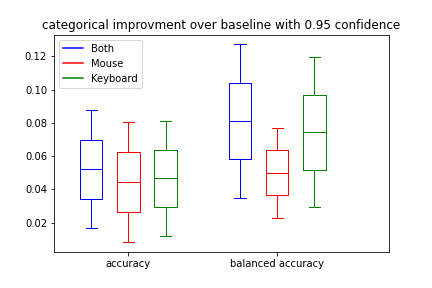
\includegraphics[width=\textwidth]{figures/results/interval_difference/1/1_categorical_0.95.png}
        \captionsetup{justification=centering}
        \caption{Confidence interval calculated for models using duration of 1 and predicting categorical labels.}
    \end{subfigure}
    \hfill
    \begin{subfigure}[b]{0.31\textwidth}
        \centering
        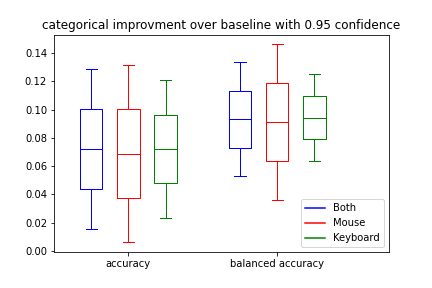
\includegraphics[width=\textwidth]{figures/results/interval_difference/5/5_categorical_0.95.png}
        \captionsetup{justification=centering}
        \caption{Confidence interval calculated for models using duration of 5 and predicting categorical labels.}
    \end{subfigure}
    \begin{subfigure}[b]{0.31\textwidth}
        \centering
        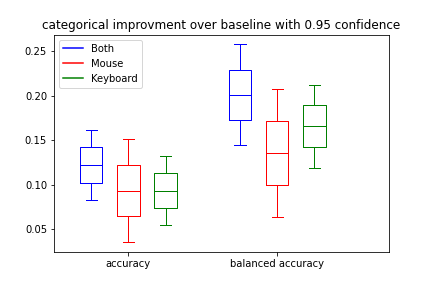
\includegraphics[width=\textwidth]{figures/results/interval_difference/10/10_categorical_0.95.png}
        \captionsetup{justification=centering}
        \caption{Confidence interval calculated for models using duration of 10 and predicting categorical labels.}
    \end{subfigure}

    %%%%%%%%%%%%%%%%%%%%%%%%%%%%%%%%%%%%%%%%%%%%% positive %%%%%%%%%%%%%%%%%%%%%%%%%%%%%%%%%%%%%%%%%%%%%

    \begin{subfigure}[b]{0.31\textwidth}
        \centering
        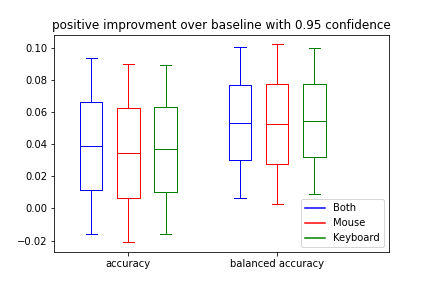
\includegraphics[width=\textwidth]{figures/results/interval_difference/1/1_positive_0.95.png}
        \captionsetup{justification=centering}
        \caption{Confidence interval calculated for models using duration of 1 and predicting positive/negative labels.}
    \end{subfigure}
    \hfill
    \begin{subfigure}[b]{0.31\textwidth}
        \centering
        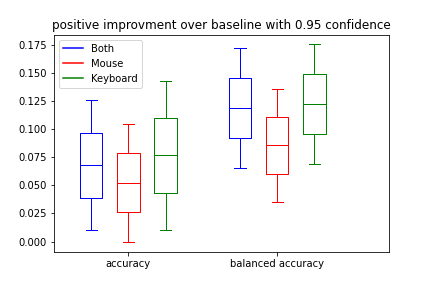
\includegraphics[width=\textwidth]{figures/results/interval_difference/5/5_positive_0.95.png}
        \captionsetup{justification=centering}
        \caption{Confidence interval calculated for models using duration of 5 and predicting positive/negative labels.}
    \end{subfigure}
    \begin{subfigure}[b]{0.31\textwidth}
        \centering
        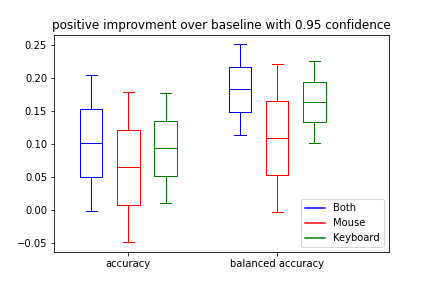
\includegraphics[width=\textwidth]{figures/results/interval_difference/10/10_positive_0.95.png}
        \captionsetup{justification=centering}
        \caption{Confidence interval calculated for models using duration of 10 and predicting positive/negative labels.}
    \end{subfigure}

    %%%%%%%%%%%%%%%%%%%%%%%%%%%%%%%%%%%%%%%%%%%%% valance %%%%%%%%%%%%%%%%%%%%%%%%%%%%%%%%%%%%%%%%%%%%%

    \begin{subfigure}[b]{0.31\textwidth}
        \centering
        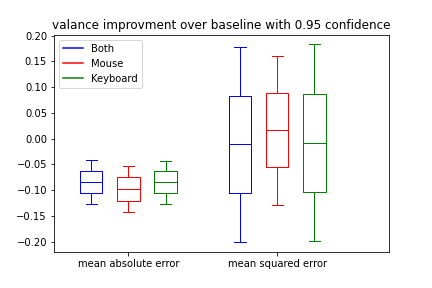
\includegraphics[width=\textwidth]{figures/results/interval_difference/1/1_valance_0.95.png}
        \captionsetup{justification=centering}
        \caption{Confidence interval calculated for models using duration of 1 and predicting valance labels.}
    \end{subfigure}
    \hfill
    \begin{subfigure}[b]{0.31\textwidth}
        \centering
        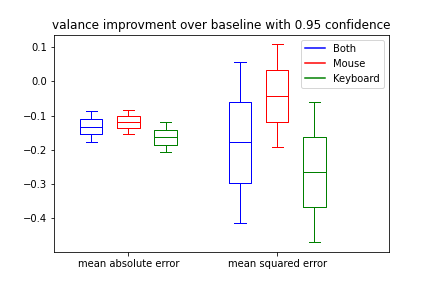
\includegraphics[width=\textwidth]{figures/results/interval_difference/5/5_valance_0.95.png}
        \captionsetup{justification=centering}
        \caption{Confidence interval calculated for models using duration of 5 and predicting valance labels.}
    \end{subfigure}
    \begin{subfigure}[b]{0.31\textwidth}
        \centering
        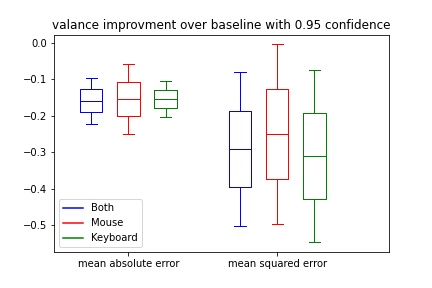
\includegraphics[width=\textwidth]{figures/results/interval_difference/10/10_valance_0.95.png}
        \captionsetup{justification=centering}
        \caption{Confidence interval calculated for models using duration of 10 and predicting valance labels.}
    \end{subfigure}

    %%%%%%%%%%%%%%%%%%%%%%%%%%%%%%%%%%%%%%%%%%%%% arousal %%%%%%%%%%%%%%%%%%%%%%%%%%%%%%%%%%%%%%%%%%%%%

    \begin{subfigure}[b]{0.31\textwidth}
        \centering
        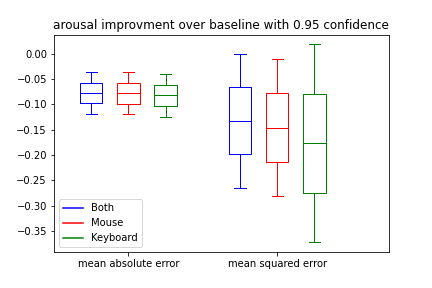
\includegraphics[width=\textwidth]{figures/results/interval_difference/1/1_arousal_0.95.png}
        \captionsetup{justification=centering}
        \caption{Confidence interval calculated for models using duration of 1 and predicting arousal labels.}
    \end{subfigure}
    \hfill
    \begin{subfigure}[b]{0.31\textwidth}
        \centering
        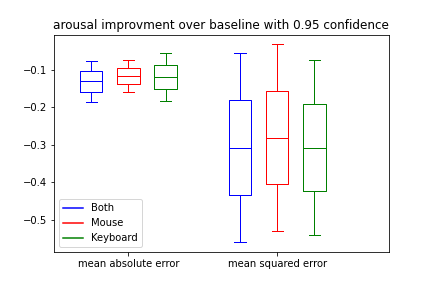
\includegraphics[width=\textwidth]{figures/results/interval_difference/5/5_arousal_0.95.png}
        \captionsetup{justification=centering}
        \caption{Confidence interval calculated for models using duration of 5 and predicting arousal labels.}
    \end{subfigure}
    \begin{subfigure}[b]{0.31\textwidth}
        \centering
        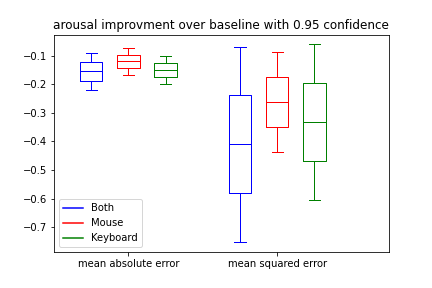
\includegraphics[width=\textwidth]{figures/results/interval_difference/10/10_arousal_0.95.png}
        \captionsetup{justification=centering}
        \caption{Confidence interval calculated for models using duration of 10 and predicting arousal labels.}
    \end{subfigure}

    %%%%%%%%%%%%%%%%%%%%%%%%%%%%%%%%%%%%%%%%%%%%% dominance %%%%%%%%%%%%%%%%%%%%%%%%%%%%%%%%%%%%%%%%%%%%%

    \begin{subfigure}[b]{0.31\textwidth}
        \centering
        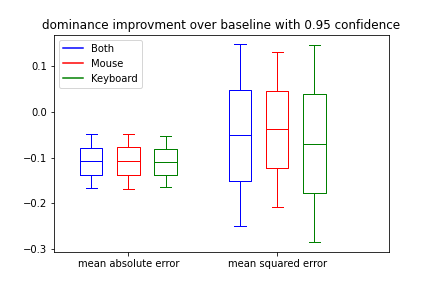
\includegraphics[width=\textwidth]{figures/results/interval_difference/1/1_dominance_0.95.png}
        \captionsetup{justification=centering}
        \caption{Confidence interval calculated for models using duration of 1 and predicting dominance labels.}
    \end{subfigure}
    \hfill
    \begin{subfigure}[b]{0.31\textwidth}
        \centering
        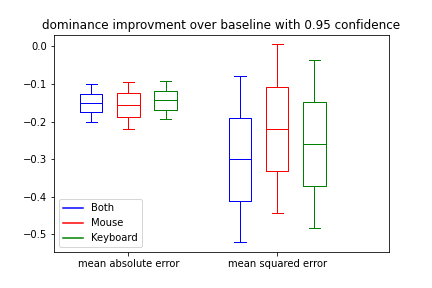
\includegraphics[width=\textwidth]{figures/results/interval_difference/5/5_dominance_0.95.png}
        \captionsetup{justification=centering}
        \caption{Confidence interval calculated for models using duration of 5 and predicting dominance labels.}
    \end{subfigure}
    \begin{subfigure}[b]{0.31\textwidth}
        \centering
        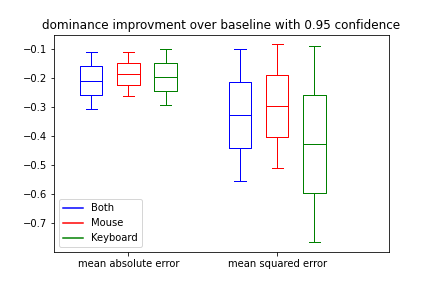
\includegraphics[width=\textwidth]{figures/results/interval_difference/10/10_dominance_0.95.png}
        \captionsetup{justification=centering}
        \caption{Confidence interval calculated for models using duration of 10 and predicting dominance labels.}
    \end{subfigure}
\end{figure}
\end{document}